% chktex-file 46
% chktex-file 3
% chktex-file 24

\section*{A. Rademacher Complexity}
\medskip

\begin{enumerate}
    \item 
    Let $\mathcal{H}$ be a set of hypotheses
    and $S$ be any sample with points $x_i$ for
    $i \in [|S|]=[m]$.
    For any $h' \in \mathcal{H}$ and any $\sigma$,
    the following inequality holds
    by the definition of supremum:
    \begin{align}
        \frac{1}{m}\sum_{i=1}^m\sigma_i h'(x_i)
        \leq \sup_{h \in \mathcal{H}}
        \frac{1}{m}\sum_{i=1}^m\sigma_i h(x_i)
        \nonumber
    \end{align}
    Then when we add over all choices of $\sigma$,
    \begin{align}
        \frac{1}{2^m} \sum_{\sigma \in \{-1,1\}^m}
        \frac{1}{m}\sum_{i=1}^m\sigma_i h'(x_i)
        &\leq 
        \frac{1}{2^m} \sum_{\sigma \in \{-1,1\}^m}
        \sup_{h \in \mathcal{H}}
        \frac{1}{m}\sum_{i=1}^m\sigma_i h(x_i)
        \nonumber \\
        \E \left[
        \frac{1}{m}\sum_{i=1}^m\sigma_i h'(x_i) \right]
        &\leq 
        \E \left[
        \sup_{h \in \mathcal{H}}
        \frac{1}{m}\sum_{i=1}^m\sigma_i h(x_i) \right]
        \nonumber
    \end{align}
    where the second inequality follows from the first
    by the definition of expectation.
    By linearity and the fact that each $\sigma_i$
    is chosen independently of $h'(x_i)$, we have
    \begin{align}
        \E \left[
        \frac{1}{m}\sum_{i=1}^m\sigma_i h'(x_i) \right]
        = \frac{1}{m} \sum_{i=1}^m \E[\sigma_i]
        \E[h'(x_i)]
        = 0
        \nonumber
    \end{align}
    since $\E[\sigma_i] = 0$ ($\sigma_i$ takes
    $1$ and $-1$ with equal probability).
    Therefore we have that
    \begin{align} 
        0 \leq 
        \E \left[
        \sup_{h \in \mathcal{H}}
        \frac{1}{m}\sum_{i=1}^m\sigma_i h(x_i) \right]
        = \hat{\mathfrak{R}}_S(\mathcal{H}).
        \nonumber   
    \end{align}
    That is, the empirical Rademacher complexity is
    non-negative.
    \item Our hypothesis set $\mathcal{H}$ is the product
    of two hypothesis sets $\mathcal{H}_1$ and $\mathcal{H}_2$.
    In mathematical notation, $h(x) = h_1(x)h_2(x)$ for some
    input $x$ where $h \in \mathcal{H}$, $h_1 \in \mathcal{H}_1$,
    and $h_2 \in \mathcal{H}_2$.

    The goal is to bound the empirical Rademacher complexity
    of $\mathcal{H}$ by the sum of the empirical Rademacher
    complexities of $\mathcal{H}_1$ and $\mathcal{H}_2$.
    The idea is to use the proof of Talagrand's contraction lemma 
    and, instead of bounding the term $\Phi \circ h(x)$ by the Lipschitz constant,
    bound $h(x)$ by $h_1(x) + h_2(x)$.

    We fix a sample $S=(x_1, \ldots, x_m)$.
    Then
    \begin{align}
        \hat{\mathfrak{R}}_S(\mathcal{H})
        &= \frac{1}{m} \E_\sigma \left[
        \sup_{h \in \mathcal{H}}
        \sum_{i=1}^m \sigma_i h(x_i)
        \right] = \frac{1}{m} \E_{\sigma_1,\ldots,\sigma_{m-1}}
        \left[ \E_{\sigma_m} \left[
        \sup_{h \in \mathcal{H}}
        u_{m-1}(h) + \sigma_m h(x_m)
        \right] \right]
        \nonumber
    \end{align}
    where $u_{m-1}(h) = \sum_{i=1}^{m-1}\sigma_i h(x_i)$.
    By definition of the supremum, for any $\epsilon>0$,
    there exist $h', h'' \in \mathcal{H}$ such that
    \begin{align}
        u_{m-1}(h') +h'(x_m)
        \geq (1-\epsilon)
        \left[
        \sup_{h \in \mathcal{H}}
        u_{m-1}(h) + h(x_m)
        \right]
        \nonumber
    \end{align}
    and 
    \begin{align}
        \label{eq:achievespp}
        u_{m-1}(h'') - h''(x_m)
        \geq (1-\epsilon)
        \left[
        \sup_{h \in \mathcal{H}}
        u_{m-1}(h) + h(x_m)
        \right].
    \end{align}
    Thus, for any $\epsilon > 0$, by definition
    of $\E_{\sigma_m}$,
    \begin{align}
        &(1-\epsilon) \E_{\sigma_m} \left[
        \sup_{h \in \mathcal{H}}
        u_{m-1}(h) - \sigma_m h(x_m)
        \right] \nonumber \\
        &= (1-\epsilon) \left[
        \frac{1}{2} \left[
        \sup_{h \in \mathcal{H}}
        u_{m-1}(h) + h(x_m)
        \right]
        + \frac{1}{2} \left[
        \sup_{h \in \mathcal{H}}
        u_{m-1}(h) - h(x_m)
        \right] \right] \nonumber \\
        &\leq \frac{1}{2}
        [u_{m-1}(h') + h'(x_m)]
        + \frac{1}{2}
        [u_{m-1}(h'') - h''(x_m)]
        \nonumber \\
        &\leq \frac{1}{2}
        [u_{m-1}(h') + u_{m-1}(h'')
        + h_1'(x_m)h_2'(x_m) - h_1''(x_m)h_2''(x_m)].
        \label{eq:preineq}
    \end{align}
    We want to show that
    \begin{align}\label{eq:inequality}
        h_1'(x_m)h_2'(x_m) - h_1''(x_m)h_2''(x_m)
        \leq h_1'(x_m) + h_2'(x_m) - (h_1''(x_m) + h_2''(x_m)).
    \end{align}
    We will prove this by cases.
    
    If $h_1'(x_m)h_2'(x_m) = 0$, then we can define $h'':=h'$
    and \autoref{eq:achievespp} still holds since $h''(x_m) \geq 0$.
    Then clearly
    \begin{align}
        h_1'(x_m)h_2'(x_m) - h_1'(x_m)h_2'(x_m)
        = 0 = h_1'(x_m) + h_2'(x_m) - (h_1'(x_m) + h_2'(x_m)).
        \nonumber
    \end{align}
    
    Otherwise, since $h_1(x_m), h_2(x_m) \in \{0,1\}$,
    we have that $h_1'(x_m)h_2'(x_m)=1$.
    If $h_1''(x_m) h_2''(x_m) = 1$, then 
    \begin{align}
        &h_1'(x_m)h_2'(x_m) - h_1''(x_m)h_2''(x_m) = 1-1 =0
        \nonumber \\
        &= 2 - 2 = h_1'(x_m) + h_2'(x_m) - (h_1''(x_m) + h_2''(x_m)).
        \nonumber
    \end{align}
    If on the other hand $h_1''(x_m) h_2''(x_m) = 0$,
    either $h_1''(x_m)=0$ or $h_2''(x_m) = 0$.
    Then either
    \begin{align}
        &h_1'(x_m)h_2'(x_m) - h_1''(x_m)h_2''(x_m) = 1-0 =1
        \nonumber \\
        &= 2 - 1 = h_1'(x_m) + h_2'(x_m) - (h_1''(x_m) + h_2''(x_m))
        \nonumber
    \end{align}
    or
    \begin{align}
        &h_1'(x_m)h_2'(x_m) - h_1''(x_m)h_2''(x_m) = 1-0 =1
        \nonumber \\
        &< 2 - 0 = h_1'(x_m) + h_2'(x_m) - (h_1''(x_m) + h_2''(x_m)).
        \nonumber
    \end{align}
    Applying \autoref{eq:inequality} to \autoref{eq:preineq}
    yields
    \begin{align}
        &(1-\epsilon) \E_{\sigma_m} \left[
        \sup_{h \in \mathcal{H}}
        u_{m-1}(h) - \sigma_m h(x_m)
        \right] \nonumber \\
        &\leq \frac{1}{2}
        [u_{m-1}(h') + u_{m-1}(h'')
        + (h_1'(x_m)+h_2'(x_m)) - (h_1''(x_m)+h_2''(x_m))]
        \nonumber \\
        &\leq \frac{1}{2}
        [u_{m-1}(h') + (h_1'(x_m)+h_2'(x_m))]
        + \frac{1}{2}
        [u_{m-1}(h'') - (h_1''(x_m)+h_2''(x_m))]
        \nonumber \\
        &\leq \frac{1}{2}
        [\sup_{h \in \mathcal{H}}
        u_{m-1}(h) + (h_1(x_m)+h_2(x_m))]
        + \frac{1}{2}[\sup_{h \in \mathcal{H}}
        u_{m-1}(h) - (h_1(x_m)+h_2(x_m))]
        \nonumber \\
        &= \E_{\sigma_m}\left[
        \sup_{h\in \mathcal{H}} u_{m-1}(h) +
        \sigma_m(h_1(x_m)+h_2(x_m))
        \right]
        \nonumber
    \end{align}
    Since the inequality holds for all $\epsilon>0$,
    we have 
    \begin{align}
        \E_{\sigma_m} \left[
        \sup_{h \in \mathcal{H}}
        u_{m-1}(h) - \sigma_m h(x_m)
        \right] \leq
        \E_{\sigma_m}\left[
        \sup_{h\in \mathcal{H}} u_{m-1}(h) +
        \sigma_m(h_1(x_m)+h_2(x_m))
        \right].
        \nonumber
    \end{align}
    Repeating the process for all other $\sigma_i$ where
    $i\neq m$ proves that
    \begin{align}
        \hat{\mathfrak{R}}_S(\mathcal{H}) \leq 
        \hat{\mathfrak{R}}_S(\mathcal{H}_1) +
        \hat{\mathfrak{R}}_S(\mathcal{H}_2).
        \nonumber
    \end{align}

\end{enumerate}

\medskip
\section*{B. VC-dimension of neural networks}
\medskip

\begin{enumerate}
    \item The goal is to bound the growth function
    $\Pi_H(m)$ in terms of the growth functions of each
    node in the intermediate layer.
    Fix $h \in H$ so that the topology of the neural
    network is set.
    We will begin by describing the growth function
    at each node.
    Since each node evaluates some $c \in C$ on $r$
    of the inputs, the growth function of a node is
    \begin{align}
        \Pi_C(m) = \max_{(x_1,\ldots, x_m)\subseteq X }
        |\{
            (c(x_1),\ldots, c(x_m)) : c\in C
        \}|.
        \nonumber
    \end{align}
    Since $c$ takes $r$ inputs, the number of features
    in $x_i$ must be at least $r$.
    Without loss of generality, $c$ evaluates
    the first $r$ features of $x_i$.

    We now consider $\Pi_H(m)$.
    Each $h \in H$ evaluates $c_0$ on $r$ points
    $u_1^{(i)},\ldots,u_r^{(i)}$ where $u_j^{(i)}=c_j(x_i)$
    for $i \in [m]$ and $j \in [r]$.
    We can assume $k=r$ by Professor Mohri's note.
    Then 
    \begin{align}
        \Pi_H(m) &= \max_{(x_1,\ldots, x_m)\subseteq X }
        |\{
            (h(x_1),\ldots, h(x_m)) : h\in C
        \}|
        \nonumber \\
        &= \sum_{(u_1,\ldots, u_r)}
        |\{
            (c_0(u_1^{(1)},\ldots,u_r^{(1)}),\ldots,
            c_0(u_1^{(m)},\ldots,u_r^{(m)})): c_0 \in C
        \}|.
        \nonumber \\
        &\leq \sum_{(u_1,\ldots, u_r) \in
        \{(c(x_1),\ldots,c(x_m)):c \in C\}^r} \Pi_C(m)
        \nonumber \\
        &= \Pi_C(m)^r \Pi_C(m) = \Pi_C(m)^{r+1}.
        \nonumber
    \end{align}

    \item The goal is to bound the VC-dimension
    of the neural networks.
    We know that the VC-dimension of $C$ is $d$.
    Sauer's Lemma gives that
    \begin{align}
        \Pi_{C}(m)\leq \sum_{i=0}^d\binom{m}{i}
        \leq \left(\frac{em}{d}\right)^d
        \nonumber
    \end{align}
    when $m \geq d$.
    (Clearly this holds since the VC-dimension of the neural networks
    is larger than the VC-dimension of $C$ by the growth
    function bound we gave.)
    Then define
    \begin{align}
        m = 2(dr + d)\log_2((dr+d)1).
        \nonumber
    \end{align}
    We will use the implication that
    $m=2x\log_2(xy) \implies m > x\log_2(ym)$
    for $m\geq 1$ and $x,y>0$ with $xy>4$.
    Then with $m=m$, $x=dr+d$, and $y=1$,
    we have
    \begin{align}
        m &> (dr+d)\log_2(m) \nonumber \\
        2^{m} &>m^{dr+d}.
        \nonumber
    \end{align}
    Define $m'=md/e$.
    Using the growth function bound and Sauer's Lemma,
    \begin{align}
        \Pi_H(m')\leq \Pi_C(m')^{r+1} \leq
        \left(\frac{em'}{d}\right)^{dr+d} = m^{dr+d} < 2^{m} \leq 2^{m'}
        \nonumber
    \end{align}
    where the last inequality holds for $d/e \geq 1$.
    Therefore the VC-dimension of the neural networks
    is bounded by
    \begin{align}
        m' = \frac{2d(dr + d)\log_2(dr+d)}{e}
        = O(d^2r\log(dr))
        \nonumber
    \end{align}
    
    \item $C$ is the family of threshold functions
    $C=\{\textrm{sgn}(\sum_{j=1}^r w_j x_j):\boldsymbol{w}\in\R^r\}$.
    The output of each hypothesis $c\in C$ is binary and
    each $c$ takes $r$ features as input so the growth function for
    any $m\geq r$ is at most $2^r$.

    We will show that the growth function of $r$ is $2^r$.
    Consider the sample of $r$ points
    $\boldsymbol{x_1},\ldots,\boldsymbol{x_r}$ where
    $\boldsymbol{x_i}$ is the zero-vector except for the $i$th
    entry which is one.
    (We use $\boldsymbol{x_i}$ to denote the $i$th sample
    and $x_j$ to denote the $j$th feature of a point.)
    Then the subset of $C$ defined such that
    $\boldsymbol{w} \in \{-1,1\}^r$
    completely shatters the $r$ points.
    To see this, observe that
    $c(\boldsymbol{x_i})=\boldsymbol{w} \cdot \boldsymbol{x_i} =w_i$.
    Then
    \begin{align}
        \Pi_C(r) = \max_{\boldsymbol{x_1},\ldots,\boldsymbol{x_r}}
        |\{ \boldsymbol{w} \cdot \boldsymbol{x_1},\ldots
        \boldsymbol{w} \cdot \boldsymbol{x_r}: \boldsymbol{w} \in \{-1,1\}^r
        \}|
        = 2^r.
        \nonumber
    \end{align}
    Together, we have that the VC-dimension of $C$ is $r$.
    (We do not include $k$ in the answer because of Professor
    Mohri's note that $k=r$.)
    Plugging in $d=r$ into the bound for the VC-dimension
    of the neural networks, we get
    \begin{align}
        \frac{2r(r^2 + r)\log_2(r^2+r)}{e}
        = O(r^3\log(r)).
        \nonumber
    \end{align}

\end{enumerate}

\medskip
\section*{C. Support Vector Machines (SVMs)}
\medskip

\begin{enumerate}
    \item Done. All my code can be found both online at
    \href{https://github.com/rtealwitter/Abalone-SVM}{github.com/rtealwitter/Abalone-SVM}
    and in the Appendix.
    \item (Insertion to keep numbering consistent.)
    \item We preprocess the data using scriptpreprocess3.py (\autoref{lst:preprocess3})
    and then scale as shown in script3.sh (\autoref{lst:script3}).
    We are careful to scale the training data then use its range
    to scale the testing data.
    \item We run cross-validation for each $d=1,2,3,4$
    $C=2^{-10},\ldots,2^{10}$ as described in script4.sh (\autoref{lst:script4}).
    We then save the accuracy with scriptextract.py (\autoref{lst:scriptextract})
    and plot the accuracy with scriptplot4.py (\autoref{lst:scriptplot4})
    as shown in \autoref{fig:4}.
    For higher values of $\log_2 C$, the error gets nearly indistinguishable.
    \begin{figure}[ht]
        \begin{center}
            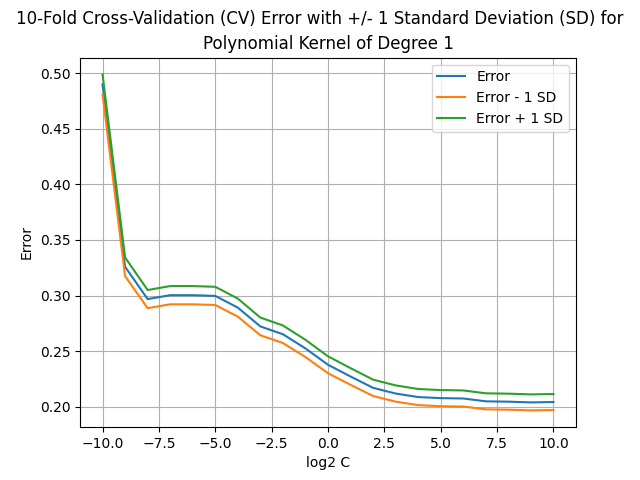
\includegraphics[width=.45\textwidth]{graphics/hw2/4.1.png}
            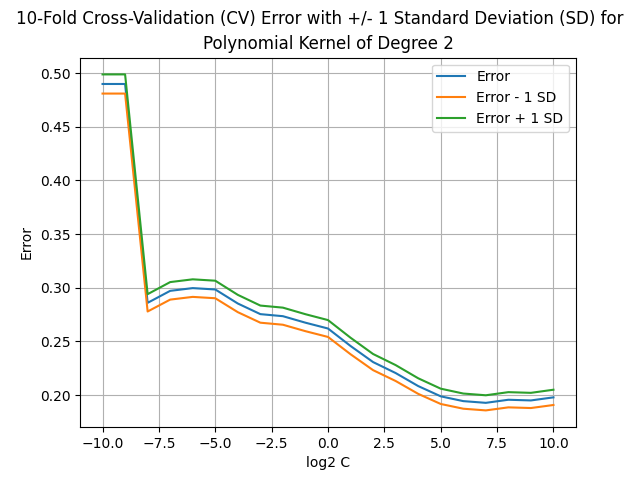
\includegraphics[width=.45\textwidth]{graphics/hw2/4.2.png}
            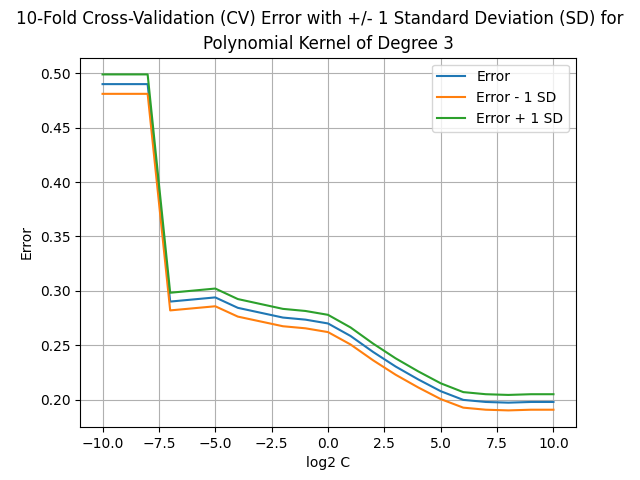
\includegraphics[width=.45\textwidth]{graphics/hw2/4.3.png}
            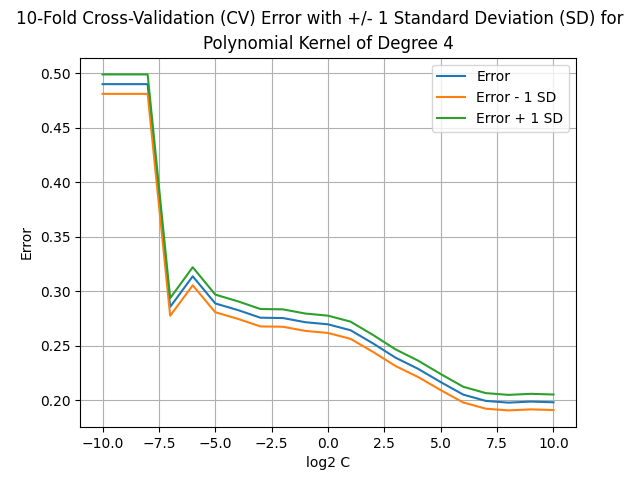
\includegraphics[width=.45\textwidth]{graphics/hw2/4.4.png}
        \end{center}
        \caption{10-fold cross-validation error of SVM with polynomial
        kernels and degree $d=1,2,3,4$ (going clockwise) plotted with
        standard deviation by values of $\log_2 C$.}
        \label{fig:4}
    \end{figure}

    \item For large $\log_2 C$, the errors are nearly indistinguishable.
    However, we achieve one of the lowest errors when $d^*=2$ and $C^*=128$.
    We set $C=128$ and use $d=1,\ldots,6$.
    We extract the accuracy again with scriptextract.py and count support vectors
    with  scriptcount.py (\autoref{lst:scriptcount}).
    We plot the testing error in \autoref{fig:5error}
    and number of support vectors in \autoref{fig:5supports}
    using scriptplot5.py (\autoref{lst:scriptplot5}).
    \begin{figure}[ht]
        \begin{center}
            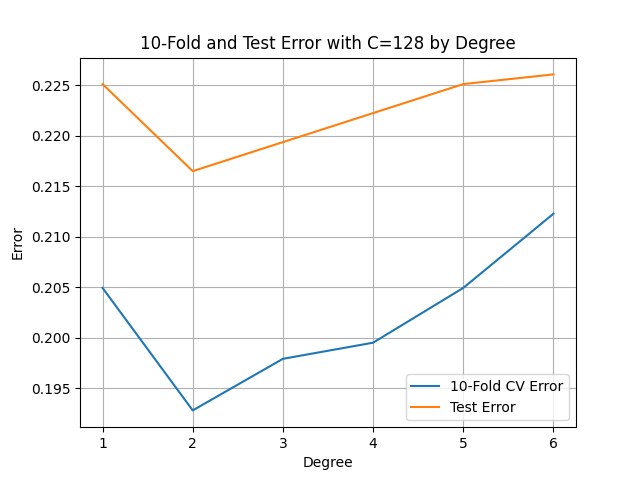
\includegraphics[width=.45\textwidth]{graphics/hw2/5error.png}
        \end{center}
        \caption{Error on 10-fold cross-validation and
        testing data as a function of degree.}
        \label{fig:5error}
    \end{figure}
    \begin{figure}[ht]
        \begin{center}
            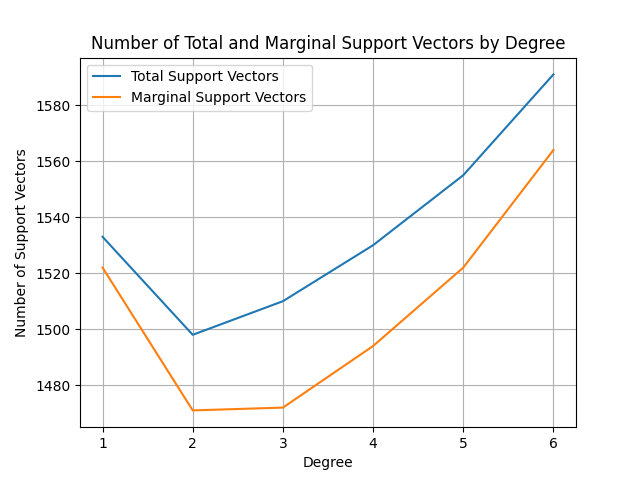
\includegraphics[width=.45\textwidth]{graphics/hw2/5supports.png}
        \end{center}
        \caption{Number of total and marginal support vectors
        as a function of degree.}
        \label{fig:5supports}
    \end{figure}

    \autoref{fig:5error} shows that the test error decreases and then
    increases with $d$.
    The error on the testing data is slightly higher than the 10-fold
    cross-validation error.
    \autoref{fig:5supports} shows that the number of total and marginal
    support vectors decreases and then increases with $d$.
 
    \item 
    The use of $\alpha$ as a coefficient in the book
    is difficult to reconcile with $\alpha$ as a sparsity vector.
    \textcolor{red}{
    Therefore we denote the sparsity vector by $a$
    and the coefficients by $\alpha'$, $\beta'$, and $\gamma'$.}
    With this notation, the optimization problem is
    \begin{align}\label{eq:primal}
        \min_{a,b} \frac{1}{2}\sum_{i=1}^m a_i^2
        + C\sum_{i=1}^m \xi_i
    \end{align}
    subject to the constraints that
    \begin{align}\label{eq:ourconstraint}
        y_i\left(
        \sum_{j=1}^m a_i y_j K(x_i,x_j)
        +b \right) \geq 1 - \xi_i
    \end{align}
    and $\xi_i,a_i\geq 0$ for $i \in [m]$.
    \begin{enumerate}
        \item The general primal optimization problem is
        equivalent to the above optimization problem except for
        the first constraint (and the non-negativity constraint
        on $a$) which, in the primal optimization problem of SVMs, is
        \begin{align}\label{eq:theirconstraint}
            y_i(a\cdot z_i + b) \geq 1 - \xi_i.
        \end{align}
        We show that, modulo the non-negativity constraint on $a$,
        the problem coincides with an instance of
        the primal optimization by constructing $z_i$
        such that \autoref{eq:ourconstraint} and
        \autoref{eq:theirconstraint} are equivalent.
        Let $z_i$ be a vector whose $j$th entry for
        $j\in[m]$ is $y_j(x_j\cdot x_i)$.
        Then
        \begin{align}
            y_i(a \cdot z_i + b) =
            y_i\left(
            \sum_{j=1}^m a_i y_j (x_i \cdot x_j)
            +b \right) = 
            y_i\left(
            \sum_{j=1}^m a_i y_j K(x_i,x_j)
            +b \right)
            \nonumber
        \end{align}
        where $K(x_i,x_j)$ is the dot product.
        Then clearly the given optimization problem and
        the following primal optimization problem of SVMs
        are equivalent:
        \begin{align}
            \min_{a,b} \frac{1}{2}\sum_{i=1}^m a_i^2
            + C\sum_{i=1}^m \xi_i
            \nonumber
        \end{align}
        subject to the constraints that
        \begin{align}
            y_i(a\cdot z_i + b)\geq 1 - \xi_i
            \nonumber
        \end{align}
        and $\xi_i\geq 0$ for $i \in [m]$
        (sans the non-negativity constraint on $a$).

        \item We answer this question by referencing
        the dual optimization problem we derive in the next question.
        The objective function of the dual is
        $G: a \rightarrow 
        -\frac{1}{2} \sum_{k=1}^m\sum_{l=1}^m \alpha_k'
        \alpha_l' y_k y_l K(x_k,x_l)
        + \frac{1}{2} \sum_{i=1}^m \gamma_i'^2
        + \sum_{i=1}^m\alpha_i'$.
        $G$ is infinitely differentiable.
        Its Hessian is given by $\nabla^2G=-K$.
        For the problem to be a convex optimization problem,
        we need $\nabla^2G$ to be concave.
        That is, $\nabla^2G \preceq 0$.
        Luckily we have this when $K$ is positive definite symmetric
        (PDS) since then $K \succeq 0$ and $-K \preceq 0$ as required.
        Therefore we need the condition that $K$ is PDS
        for \autoref{eq:primal} to be a convex optimization problem.

        \item \textcolor{red}{Important: to reconcile the notation of
        the book and problem, we use $a$ to represent the
        sparsity vector we want to minimize and $\alpha_i'$,
        $\beta_i'$ and $\gamma_i'$ to represent coefficients
        in the optimization problem.}

        The Lagrangian is
        \begin{align}
            L(a, b, \xi, \alpha', \beta', \gamma')
            &= \frac{1}{2}{\norm{a}^2} + C \sum_{i=1}^m\xi_i
            - \sum_{i=1}^m\alpha_i'(y_i(\sum_{j=1}^m a_j y_j x_j
            \cdot x_i + b)-1 + \xi_i) \nonumber \\
            &- \sum_{i=1}^m\beta_i'\xi_i - \sum_{i=1}^m\gamma_i'a_i
            \nonumber \\
            &= \frac{1}{2}{\norm{a}^2} + C \sum_{i=1}^m\xi_i
            - (\sum_{i=1}^m\alpha_i'y_i x_i)
            (\sum_{j=1}^m a_j y_j x_j) \nonumber \\
            &- \sum_{i=1}^m\alpha_i'y_i b + \sum_{i=1}^m\alpha_i'
            - \sum_{i=1}^m\alpha_i'\xi_i
            - \sum_{i=1}^m\beta_i'\xi_i - \sum_{i=1}^m\gamma_i'a_i.
            \nonumber
        \end{align}
        Then the KKT conditions yield
        \begin{align}
            \nabla_{a_i}L &= a_i - y_i x_i \sum_{k=1}^m
            \alpha_k'y_k x_k - \gamma_i' = 0
            \label{eq:kkta} \\
            \nabla_{b}L &= -\sum_{i=1}^m\alpha_i' y_i = 0
            \label{eq:kktb} \\
            \nabla_{\xi_i}L &= C - \alpha_i' - \beta_i' = 0
            \label{eq:kktxi}
        \end{align}
        subject to the constraints that
        \begin{align}
            \alpha_i'(y_i(\sum_{j=1}^m a_j y_j x_j\cdot x_i
            + b) -1 +\xi_i) 
            =\beta_i'x_i
            =\gamma_i'a_i=0
            \nonumber
        \end{align}
        for $i \in [m]$.
        Now we simplify the Lagrangian with the
        new information:
        \begin{align}
            L &= \frac{1}{2}\norm{a}^2 + C\sum_{i=1}^m
            - \sum_{i=1}^m a_i(a_i-\gamma_i')
            - b\sum_{i=1}^m\alpha_i'y_i \nonumber \\
            &+ \sum_{i=1}^m\alpha_i' -\sum_{i=1}^m \alpha_i' \xi_i
            - \sum_{i=1}^m\beta_i' \xi_i - \sum_{i=1}^m a_i \gamma_i'.
            \nonumber
        \end{align}
        We use the following expressions:
        $y_i x_i \sum_{k=1}^m \alpha_k'y_k x_k = a_i -\gamma_i'$
        from \autoref{eq:kkta},
        $\alpha_i'+\beta_i'=C$ from \autoref{eq:kktb}, and
        $\sum_{i=1}^m \alpha_i'y_i=0$ from \autoref{eq:kktxi}.
        Then we simply have
        \begin{align}
            L=-\frac{1}{2}\norm{a}^2 + \sum_{i=1}^m \alpha_i'.
            \nonumber
        \end{align}
        Unfortunately $\norm{a}^2$ is not so simple:
        \begin{align}
            \norm{a}^2 &= \sum_{i=1}^m(y_i x_i
            \sum_{k=1}^m \alpha_k' y_k x_k +\gamma_i')^2
            \nonumber \\
            &= \sum_{i=1}^m [(y_i x_i \sum_{k=1}^m \alpha_k' y_k x_k)^2
            + \gamma_i'^2 + 2\gamma_i y_i x_i \sum_{k=1}^m \alpha_k' y_k x_k].
            \nonumber
        \end{align}
        Here, we get lucky since we know $\gamma_i'a_i = 0$
        from the constraints on the KKT conditions so
        $\gamma_i'(y_i x_i \sum_{k=1}^m \alpha_k' y_k x_k +\gamma_i')=0$
        and
        $\gamma_i'^2 = -\gamma_i'y_i x_i \sum_{k=1}^m \alpha_k' y_k x_k$.
        Then 
        \begin{align}
            &= \sum_{i=1}^m[y_i^2 x_i^2 \sum_{k=1}^m\alpha_k'y_k x_k
            \sum_{l=1}^m\alpha_l'y_l x_l + \gamma_i'^2 - 2\gamma_i'^2]
            \nonumber \\
            &= \sum_{k=1}^m\sum_{l=1}^m \alpha_k'\alpha_l' y_k y_l
            \sum_{i=1}^m(x_i y_i x_k) (x_i y_i x_l)
            - \sum_{i=1}^m \gamma_i'^2 \nonumber \\
            &= \sum_{k=1}^m\sum_{l=1}^m \alpha_k'\alpha_l' y_k y_l K(x_k,x_l)
            - \sum_{i=1}^m \gamma_i'^2 \nonumber.
        \end{align}
        We combine our expression for $\norm{a}^2$ with 
        our expression for $L$.
        We have that the dual optimization problem is
        \begin{align}
            \max_{\alpha', \gamma'}
            -\frac{1}{2} \sum_{k=1}^m\sum_{l=1}^m \alpha_k'\alpha_l' y_k y_l K(x_k,x_l)
            + \frac{1}{2} \sum_{i=1}^m \gamma_i'^2
            + \sum_{i=1}^m\alpha_i'
            \nonumber
        \end{align}
        subject to the constraints that $0 \leq \alpha_i' \leq C$
        (since $\beta_i'\geq0$ and $\beta_i'+\alpha_i'=C$) and
        $\sum_{i=1}^m\alpha_i'y_i=0$ for $i \in [m]$.
        (Clearly any real $\gamma_i'$ suffices because then
        $\gamma_i'^2$ has to be non-negative which is what we need.)

        \item We transform the data into the sparsity minimization problem
        using the $z_i$ constraint transformation in \autoref{eq:theirconstraint}
        via scriptpreprocess6.py (\autoref{lst:preprocess6}).
        We then scale the data, making sure to use the range of the training
        data for both the training and test data.
        Next, we identify good values of $C$.
        Again, the error becomes almost indistinguishable but one of the best
        values is $C^*=32$.
        We then calculate the error
        rates of 10-fold cross-validation and the test data.
        We plot the data with scriptplot6.py (\autoref{lst:scriptplot6}).
        \autoref{fig:6error} shows the error of the 10-fold cross-validation
        roughly increases with $d$ while the error on the testing data
        roughly decreases.
        The errors are approximately the same for $d\leq3$ but for $d\geq4$ the
        test error is surprisingly smaller.
        The whole approach can be found in script6.sh (\autoref{lst:script6}).
        \begin{figure}[ht]
            \begin{center}
                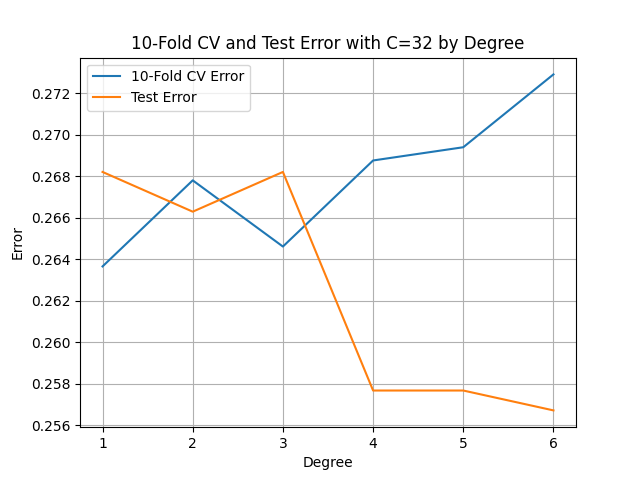
\includegraphics[width=.45\textwidth]{graphics/hw2/6error.png}
            \end{center}
            \caption{Error on 10-fold cross-validation and
            testing data as a function of degree.}
            \label{fig:6error}
        \end{figure} 


    \end{enumerate}
\end{enumerate}

\appendix
\section*{Appendix}
\lstinputlisting[label={lst:script3}, language=Bash, caption={Scaling training data and then using training range to scale test data.}]{code/hw2/script3.sh}
\lstinputlisting[label={lst:preprocess3}, language=Python, caption={Preprocessing abalone.data.}]{code/hw2/scriptpreprocess3.py}
\lstinputlisting[label={lst:script4}, language=Bash, caption={Finding good $d$ and $C$ parameters via 10-fold cross-validation accuracy.}]{code/hw2/script4.sh}
\lstinputlisting[label={lst:scriptextract}, language=Python, caption={Extract accuracy parameter.}]{code/hw2/scriptextract.py}
\lstinputlisting[label={lst:scriptplot4}, language=Python, caption={Plot error rate as a function of $\log_2 C$.}]{code/hw2/scriptplot4.py}
\lstinputlisting[label={lst:script5}, language=Bash, caption={Error rate on 10-fold cross-validation and testing in addition to number of total and marginal support vectors.}]{code/hw2/script5.sh}
\lstinputlisting[label={lst:scriptcount}, language=Python, caption={Count the number of total and marginal support vectors.}]{code/hw2/scriptcount.py}
\lstinputlisting[label={lst:scriptplot5}, language=Python, caption={Plot error of 10-fold cross-validation and testing data as well as total and marginal support vectors by degree.}]{code/hw2/scriptplot5.py}
\lstinputlisting[label={lst:script6}, language=Bash, caption={Scaling data, finding a good $C$, and finding and plotting error.}]{code/hw2/script6.sh}
\lstinputlisting[label={lst:preprocess6}, language=Python, caption={Transform data into sparsity minimization problem.}]{code/hw2/scriptpreprocess6.py}
\lstinputlisting[label={lst:scriptplot6}, language=Python, caption={Plot error of 10-fold cross-validation and testing data.}]{code/hw2/scriptplot6.py}

